\section{System's Perspective}
\label{ch:sys_persp} % used to ref this chapter

This section covers the main modules of the system with their  
respective technologies and dependencies, as well as how they
were deployed.

\subsection{Module view}

\begin{figure}[H]
    \centering
    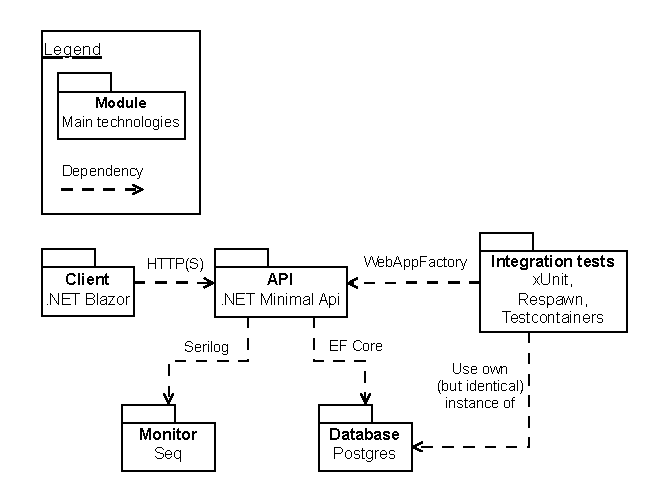
\includegraphics[width=\linewidth]{images/modules.drawio.pdf}
    \caption{Diagram showing the modules that make up the system with
    their dependencies and main technologies.}
    \label{fig:modules}
\end{figure}

Figure \ref{fig:modules} provides an overview of how the main modules are connected, specifically:
\begin{itemize}
    \item Users interact with the \texttt{Client} module
    \item The \texttt{Client} module sends requests to the \texttt{API} module which contains a \texttt{PostgreSQL} database connection
    \item The \texttt{Monitor} module reads logs written by the \texttt{API}
    \item The \texttt{Integration tests} module uses services from the \texttt{API} and its own database instance to test the \texttt{API}
\end{itemize}

\subsection{Deployment view}

\begin{figure}[H]
      \centering
      \makebox[\linewidth]{
      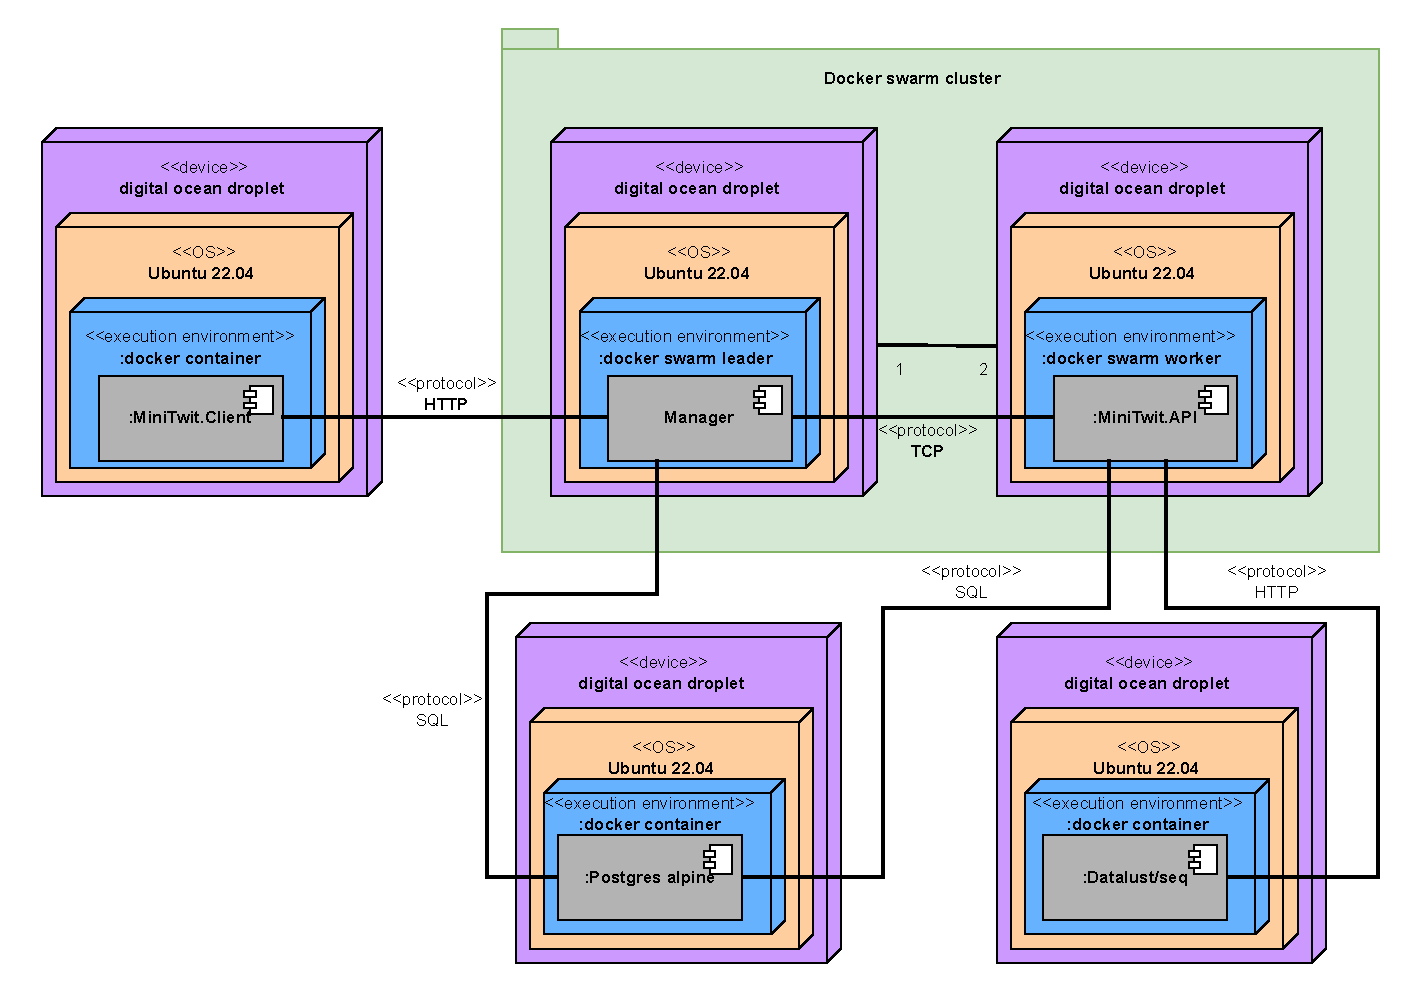
\includegraphics[width=1.4\textwidth]{images/deployment_diagram.drawio.pdf}}
      \caption{Deployment diagram showing how the modules were deployed.}
      \label{fig:deployment_diagram}
\end{figure}

We use \texttt{Digital Ocean} to deploy the respective modules to \texttt{droplets} running \texttt{Ubuntu 22.04} as illustrated in Figure \ref{fig:deployment_diagram}. 
It works by creating and pushing \texttt{Docker} images which each \texttt{droplet} can pull and run.

\subsection{\texttt{API}}

The \texttt{API} functions as the backend for our \texttt{MiniTwit} application.
It is deployed as three separate units to form a \texttt{Docker Swarm}. 
One is the \texttt{leader/manager} giving tasks to 
the two others, who act as \texttt{workers}. 
Thus, the \texttt{leader} functions as a \texttt{load balancer} using the \texttt{workers} as servers.
We decided that the \texttt{leader} should not be a \texttt{worker},
because we wanted it to function optimally as a \texttt{load balancer}.
We were not sure how it would be affected by also acting as a \texttt{worker}.
Instead, we can use it to run other side tasks, like \texttt{database migrations}.

The \texttt{API} project is implemented in \texttt{.NET} using \texttt{Minimal API}\cite{minimalApi}.
The \texttt{database} communication is done using \texttt{Entity Framework Core}.
It logs using \texttt{Serilog}\cite{serilog}, 
which is configured to write to \texttt{Seq}\cite{seq}.

\subsection{\texttt{Client}}

The \texttt{Client} is the frontend for the \texttt{MiniTwit} application implemented as a \texttt{Blazor WebAssembly} app. 
This way the workload is distributed to the users' browsers rather than a server. It is responsible for sending requests and 
receiving responses from the \texttt{API} module.

\subsection{Monitor}

Our \texttt{Monitor} uses the tool \texttt{Seq}\cite{seq}.
It handles logs and displays custom graphs based on 
the log information. We have both developer-relevant 
graphs such as \texttt{API} response times and errors,
as well as business-relevant graphs such as number 
of newly registered users and messages posted.
It is deployed on its own \texttt{Digital Ocean} \texttt{droplet} 
using an image provided by \texttt{Datalust}\cite{seq}.

\subsection{Database}

The \texttt{database} is a \texttt{PostgreSQL}\cite{postgres} database.
It contains information about registered users,
posted messages, and followers.

\subsection{Sequence diagram}

\begin{figure}[H]
    \centering
    \makebox[\linewidth]{
    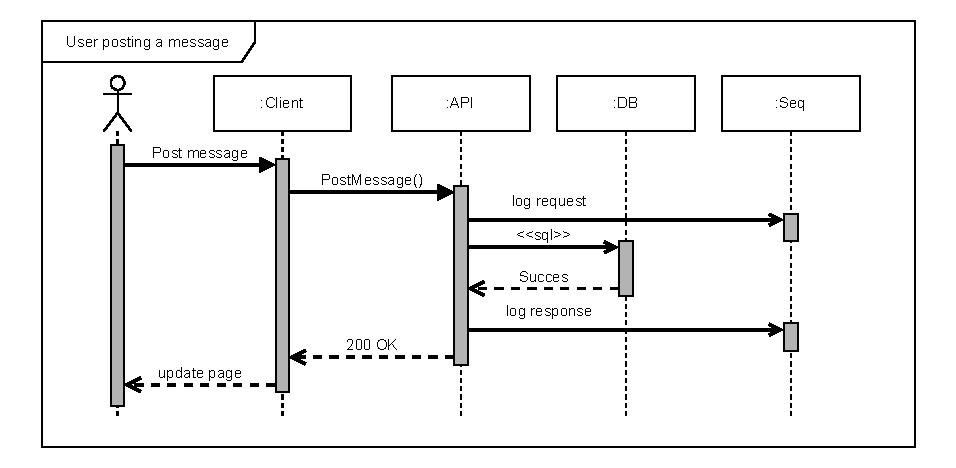
\includegraphics[width=1.4\textwidth]{images/sequence_diagram.drawio.pdf}}
    \caption{Sequence diagram showing how the system acts upon 
    a user successfully posting a message.}
    \label{fig:seq_diagram}
\end{figure}

In summary, users post messages from the \texttt{Client}.
The \texttt{Client} sends requests to the \texttt{API}, which logs the request 
information, saves the messages to the database, 
logs the response information, and sends responses back to the 
\texttt{Client}. Logs are used for monitoring in \texttt{Seq}. 
The \texttt{Client} then updates the \texttt{UI} for the users.
This is illustrated in Figure \ref{fig:seq_diagram}.
